\documentclass[tikz,border=6pt]{standalone}
\usepackage{pgfplots}
\usepgfplotslibrary{groupplots}
\usetikzlibrary{calc}
\pgfplotsset{compat=1.18}
\begin{document}
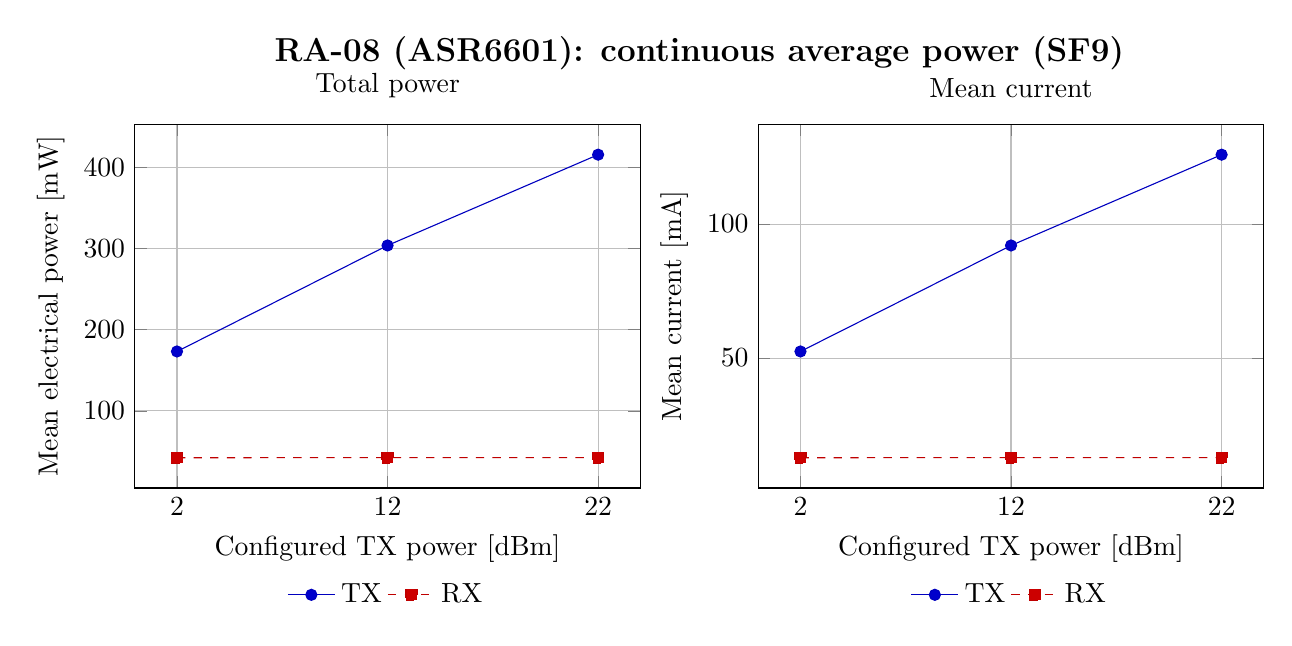
\begin{tikzpicture}
\begin{groupplot}[group style={group size=2 by 1,horizontal sep=1.5cm},width=8cm,height=6.2cm,xtick={2,12,22},xlabel={Configured TX power [dBm]},grid=both,legend style={draw=none,at={(0.5,-0.23)},anchor=north,legend columns=2}]
\nextgroupplot[title={Total power},ylabel={Mean electrical power [mW]}]
\addplot+[blue!75!black,mark=*] coordinates {(2,173.147341) (12,303.637739) (22,415.427325)};\addlegendentry{TX}
\addplot+[red!75!black,dashed,mark=square*] coordinates {(2,42.3241632) (12,42.4136083) (22,42.3978593)};\addlegendentry{RX}
\nextgroupplot[title={Mean current},ylabel={Mean current [mA]}]
\addplot+[blue!75!black,mark=*] coordinates {(2,52.4688912) (12,92.0114362) (22,125.887068)};\addlegendentry{TX}
\addplot+[red!75!black,dashed,mark=square*] coordinates {(2,12.825504) (12,12.8526086) (22,12.8478361)};\addlegendentry{RX}
\end{groupplot}
\node[font=\bfseries\large] at ($(group c1r1.north)!0.5!(group c2r1.north)+(0,0.9cm)$) {RA-08 (ASR6601): continuous average power (SF9)};
\end{tikzpicture}
\end{document}
